\documentclass{article}
\usepackage{changepage}
\usepackage{float}
\usepackage{amsmath}
\usepackage{tikz}
\usepackage{graphicx}
\usepackage{color}
\usepackage{listings}
\usetikzlibrary{arrows}

\long\def\/*#1*/{}

\tikzset{
  treenode/.style = {align=center, inner sep=0pt, text centered,
    font=\sffamily},
  1/.style = {treenode, circle, white, font=\sffamily\bfseries, draw=black,
    fill=black, text width=1.5em},% arbre rouge noir, noeud noir
  2/.style = {treenode, circle, white, draw=black, 
    text width=1.5em, very thick},% arbre rouge noir, noeud rouge
  %3/.style = {treenode, circle, white, draw=black,
    %minimum width=0.5em, minimum height=0.5em}% arbre rouge noir, nil
}

\begin{document}
\begin{center}
Andreas Landgrebe \\
Computer Science 250 \\
Laboratory Assignment 4 \\
Improving Standard Sorting Algorithms \\
February 11, 2015 \\
\end{center}
\newpage
\begin{center}
\textbf{Part 1 Results}
\end{center}

\begin{figure}[H]
\centering
\begin{adjustwidth}{-3.4cm}{}
\begin{tabular}{| l | l | l | l | l | l | l | l |}
\hline
Altering Insertion Sort & Run 1 & Run 2 & Run 3 & Run 4 & Run 5 & Mean(Average) & Standard Deviation\\ \hline
Array Length 1000 & 5.043 & 4.870 & 5.522 & 4.913 & 5.571 & 5.1838 & 0.30197046213165 \\ \hline
Array Length 10000 & 429.310 & 461.410 & 408.542 & 449.632 & 448.370 & 434.47566667 & 20.102257896952 \\ \hline
Array Length 100000 & 10280.331 & 10831.381  & 10269.832 & 10199.987 & 10596.183  & 10435.5428 & 240.63684732177 \\ \hline
\end{tabular}
\caption{Results of NewInsertion vs Insertion}
\end{adjustwidth}
\end{figure}

\includegraphics[scale=0.75]{NewInsertion.png}

\newpage

\begin{center}
\textbf{Part Two Results}
\end{center}

\begin{figure}[H]
\centering
\begin{adjustwidth}{-3.4cm}{}
\begin{tabular}{| l | l | l | l | l | l | l | l |}
\hline
Altering Mergesort & Run 1 & Run 2 & Run 3 & Run 4 & Run 5 & Mean(Average) & Standard Deviation\\ \hline
Threshold Value 5 & 1.249 & 1.258 & 1.276 & 1.295 & 1.288 & 1.2732 & 0.017428711943227\\ \hline
Threshold Value 10 & 1.583 & 1.541 & 1.496 & 1.569 & 1.561 & 1.55 & 0.0302258167797\\ \hline
Threshold Value 25 & 2.042 & 1.942 & 2.060 & 2.025 & 2.051 & 2.024 & 0.042600469480981\\ \hline
Threshold Value 100 & 3.031 & 3.014 & 3.111 & 2.025 & 2.051 & 2.6464 & 0.49790344445485\\ \hline
\end{tabular}
\caption{Results of MergeInsertion vs Merge with different threshold vaues}
\end{adjustwidth}
\end{figure}

\includegraphics[scale=0.75]{MergeInsertion.png}

\newpage

\begin{center}
\textbf{Part 3 Results}
\end{center}
\begin{figure}[H]
\centering
\begin{adjustwidth}{-3.4cm}{}
\begin{tabular}{| l | l | l | l | l | l | l | l |}
\hline
Altering Quicksort & Run 1 & Run 2 & Run 3 & Run 4 & Run 5 & Mean(Average) & Standard Deviation\\ \hline
Array Length 10000 & 0.880 & 0.801 & 0.831 & 0.832 & 0.924 & 0.8536 & 0.043352508577936 \\ \hline
Array Length 100000  & 1.014 & 1.007 & 1.028 & 0.930 & 0.943 & 0.9844 & 0.039902882101422\\ \hline
Array Length 1000000  & 1.090 & 1.012 & 0.990 & 1.152 & 1.032 & 1.0552 & 0.05871422314908 \\ \hline
\end{tabular}
\caption{Results of Three QuickSort vs QuickSort}
\end{adjustwidth}
\end{figure}

\includegraphics[scale=0.75]{ThreeQuickSort.png}

\newpage

\begin{center}
\textbf{Part 4: While You Have Some Downtime}
\end{center}
\begin{enumerate}
\item Trace how the Heapsort algorithm will sort the array REHEAPIFICATION
\begin{center}
\textbf{1. Build the heap}
\end{center}
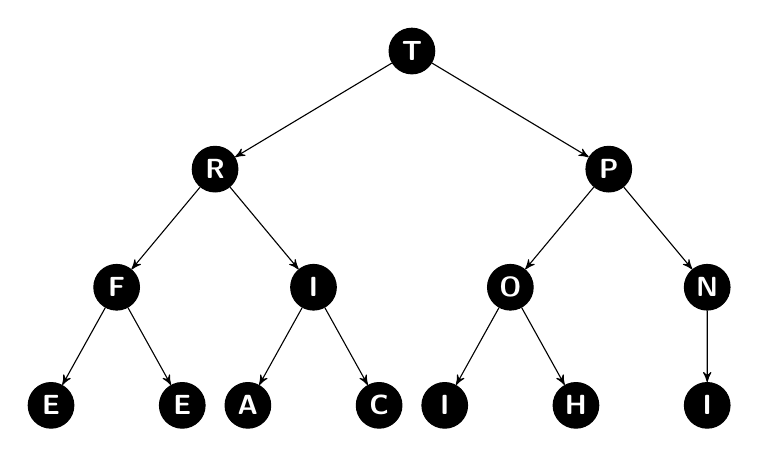
\begin{tikzpicture}[->,>=stealth',level/.style={sibling distance = 5cm/#1,
  level distance = 1.5cm}] 
\node [1] {T}
    child{ node [1] {R} 
            child{ node [1] {F} 
            	child{ node [1] {E} edge from parent node[above left]
                         {}} %for a named pointer
							child{ node [1] {E}}
            }
            child{ node [1] {I}
							child{ node [1] {A}}
							child{ node [1] {C}}
            }                            
    }
    child{ node [1] {P}
            child{ node [1] {O} 
							child{ node [1] {I}}
							child{ node [1] {H}}
            }
            child{ node [1] {N}
							child{ node [1] {I}}
							%child{ node [3] {}}
            }
		}
; 
\end{tikzpicture}
\begin{center}
\textbf{2. Sorting}
\end{center}
TRPFIONEEACIHI\\
IRPFIONEEACIHI\\
IRPFIONEEACIH Sorting Array: T\\
RIPFIONRRACIH\\
HIPFIONRRACIR\\ Sorting Array: TR\\
PIHFIONRRACIR\\
PIOFIHNEEACI\\
PIOFIINRRACH\\
HIOFIINEEAC Sorting Array: TRP\\
OIHFIINEEAC\\
OINFIIHEEAC\\
CINFIIHEEA Sorting Array: TRPO \\
NICFIIHEEA \\
NIIFICHEEA\\
AIIFICHEE Sorting Array: TRPON\\
IAIFICHEE \\
IIIFACHEE\\
EIIFACHE Sorting Array: TRPONI\\
IEIFACHE \\
IFIEACHE \\
EFDIEACH Sorting Array: TRPONII\\
IFEEACH \\
IFHEACE \\
EFHEAC Sorting Array: TRPONIII \\
HFEEAC \\
CFEEA Sorting Array: TRPONIIIH \\
FCEEA \\
FEECA \\
AEEC Sorting Array: TRPONIIIHF \\
EAEC \\
ECEA \\
ACE Sorting Array: TRPONIIIHFE \\
EAC \\
AC Sorting Array: TRPONIIIHFEE \\
CA \\
A Sorting Array: TRPONIIIHFEEC \\
Sorting Array: TRPONIIIHFEECA \\




\item What is the minimum number of items that must be exchanged during a \textbf{RemoveMax()} operation on a heap of size N? Give a heap of size 15 for which this minimum is achieved. 
Of a heap size n, the minimum number of items that must be exchanged is 2.

\end{enumerate}
\end{document}